\setcounter{mtc}{5} %indique le numero reel du chapitre, pour la mini table des matieres
\chapter{Project Scope}
\minitoc  %insert la minitoc

\graphicspath{{Chapitre1/figures/}}
%==============================================================================
\pagestyle{fancy}
\fancyhf{}
\fancyhead[R]{\bfseries\rightmark}
\fancyfoot[R]{\thepage}
\renewcommand{\headrulewidth}{0.5pt}
\renewcommand{\footrulewidth}{0pt}
\renewcommand{\chaptermark}[1]{\markboth{\MakeUppercase{\chaptername~\thechapter. #1 }}{}}
\renewcommand{\sectionmark}[1]{\markright{\thechapter.\thesection~ #1}}

\begin{spacing}{1.2}
%==============================================================================

\section*{Introduction}
This chapter is dedicated to the presentation of our project's general scope. 
This will include an introduction of the host company Kaoun and it's main product Flouci. Also we will give an overview of the developer API project. After that, we will describe the chosen methodology that we followed during the realization of our project.
\section{Host company presentation} 
In The first section of the report, we will introduce Kaoun, The host company that made the project possible.
\subsection{Presentation of Kaoun}
Kaoun is a new FinTech company that builds reliable infrastructure for payments and credits in Tunisia, and whose mission is to enable all individuals and businesses to access financial services using any phone, anywhere, anytime. 

Kaoun's first product, Flouci, is a mobile and web payment application built on top of a unique decentralized inter and intrabank infrastructure that allows instant transactions for peer to peer transfers and merchant payments. Kaoun plans to work with governments, traditional banks, mobile operators, and microfinance institutions to fix the lag between technology adoption and financial inclusion by reducing the barriers to entry for the unbanked and the underbanked.


\begin{figure}[!ht]\centering

\includegraphics[scale=0.3]{kaounlogo.png}
\caption{Kaoun logo}
\label{fig:fig1}
\end{figure}


\subsection{Presentation of Flouci}
Flouci is the first wallet designed to innovate mobile payment in Tunisia. It serves as a quick, easy, and convenient way to open a bank account, send and receive money, and pay different merchants in-person or online, all from within the app. 
\begin{itemize}
  \item \textbf{Open an account:}
  
  In order to create a Flouci account, you either link your Flouci wallet to an existing bank account or follow the step-by-step KYC (Know Your Customer) guide to create an account with one of our partner financial institutions. Once you have your wallet and your QR code, you can start sending and receiving money and paying merchants using your phone. 

  \item \textbf{Send and receive money:}
  
  Once you create a Flouci account, you can send and receive money to and from anybody that has a flouci account/wallet. It's easy, cheap, and secure. And the best part is that it's practically instant. All you have to do is enter their number or scan their personal QR code to access their profile. You then enter the amount and confirm. You both then receive a confirmation SMS and you're done.
  \item \textbf{Pay merchants:}
  
  Through Flouci, you have access to a wide range of partner merchants across Tunisia. You can pay through the app by just scanning the QR code shown on the counter of the merchant. No waiting lines, no more looking for change or realizing you forgot your wallet at home. 
\end{itemize}

\begin{figure}[!ht]\centering

\includegraphics[scale=0.3]{floucilogo.png}
\caption{Flouci logo}
\label{fig:fig1}
\end{figure}

\section{Project overview}
In this section, we will present the developer API project context, we will analyze some of the existing mobile payments API's. And finally, we will indicate our project goals.
\subsection{Project Context}
Flouci in it's first version made it possible for users to pay merchants in simple steps and without the need of cash. However the market is rapidly shifting toward online e-commerce sites with companies like Jumia, Tayara and many other introducing their solutions in Tunisia.

In it's current implementation Flouci is not able to integrate into any form of online payments due to the lack of it's implementation.

Facing this problem and a fast moving e-commerce market the company had to move toward implementing a solution for developers.

The API should make it possible for developers to link their Flouci wallets to the their e-commerce sites and add flouci as an easy and instant payment method.
\subsection{Study of the existing}
In The world of e-commerce a lot of payments methods exists. Most of the methods are credit card related and offer the possibility to pay using the card number and the 3 digits code. 

In our case Flouci offer payments through QR codes scans. Although the payment steps on the user side is different the developer API should offer similar functionalities.


Below is a list of world leader online payment API's:
\begin{itemize}
  \item \textbf{Stripe:}
 
 The Stripe API is organized around REST. The API has predictable resource-oriented URLs, accepts form-encoded request bodies, returns JSON-encoded responses, and uses standard HTTP response codes, authentication, and verbs.

You can use the Stripe API in test mode, which does not affect your live data or interact with the banking networks. The API key you use to authenticate the request determines whether the request is live mode or test mode.

\begin{figure}[!ht]\centering
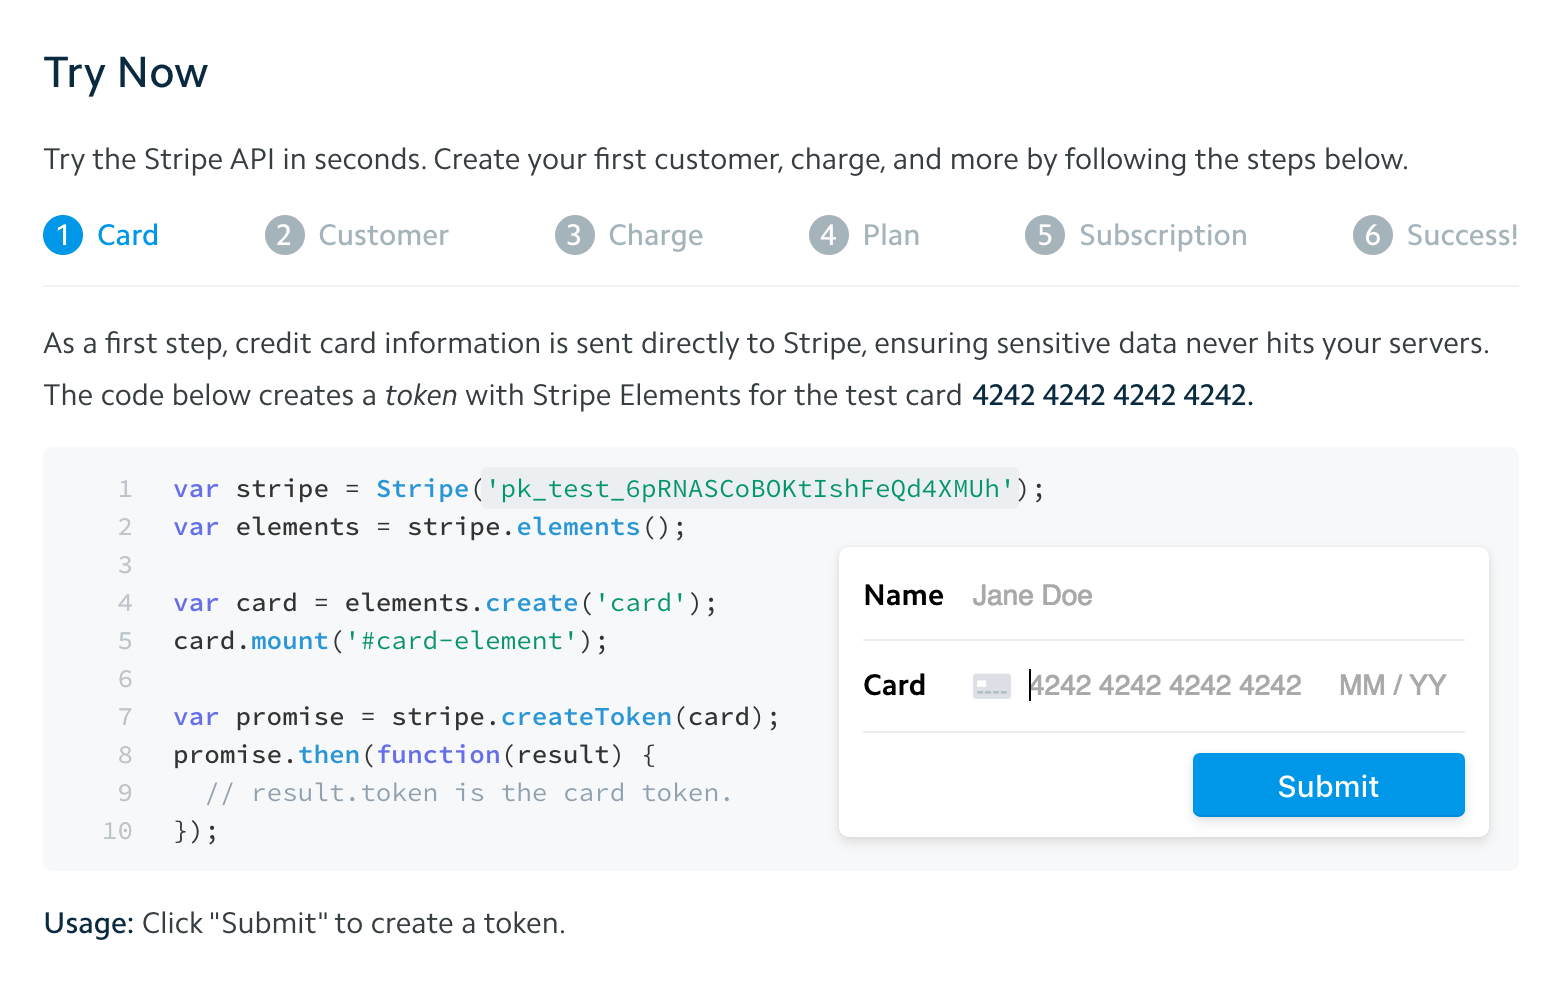
\includegraphics[scale=0.3]{stripe.png}
\caption{Stripe Api}
\label{fig:fig1}
\end{figure}

  \item \textbf{Paypal:}
  
  The PayPal APIs are HTTP-based RESTful APIs that use OAuth 2.0 for authorization. API request and response bodies are formatted in JSON.
  
\begin{figure}[!ht]\centering
\includegraphics[scale=0.3]{PayPal.png}
\caption{Stripe Api}
\label{fig:fig1}
\end{figure}
\newpage
\item \textbf{Twint:}

Twint is the closest implementation to Flouci, it offers payments through QR code scans.

The plugin allows QR code generation on the web page, it also creates a code for each transaction, It serves to confirm payments.
\begin{figure}[!ht]\centering
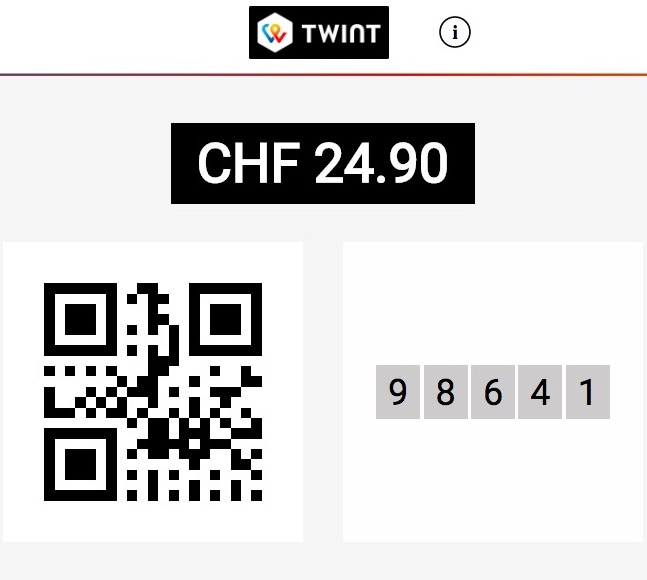
\includegraphics[scale=0.3]{twint.jpg}
\caption{Twint Payment Method}
\label{fig:fig1}
\end{figure}
  \end{itemize}

\subsection{Project goals}
To bring developers to the Flouci world and allow e-commerce owners to introduce a mobile payment solution Kaoun has decided to build it's own developer API from scratch and provide an easy way to accept payments in few simple steps. This presented the opportunity for us to turn this problem into the main objective of our graduation project.

By the end of our project, we need to achieve these goals :
\begin{itemize}
  \item \textbf{Create Account:}
  
  Any developer should be able to create a Flouci developer account from the web platform, basic informations are needed to open an account.
  
  Also it should be possible to use an existing Flouci account and switch it to developer mode.
   
  \item \textbf{Create App and link Flouci wallet:}

  The web interface should offer the possibility to create an App and link an existing wallet to the specific configuration. A two steps verification system should be put in place to verify ownership of the wallet.
  To verify transaction developer could choose between two modes:
  \begin{itemize}
  \item \textbf{Active mode:} Activate an endpoint to verify transactions by id.
  \item \textbf{Passive mode:} Configure a webhook to receive transactions info once validated.
   \end{itemize}
   A unique token is generated for each app to allow client integration.
  \item \textbf{Integrate Flouci client:}
 
 Once the App is configured the developer can easily add flouci as a payment method with the token provided.
  \item \textbf{Check App analytics:}
  
  Every App should enable a dashboard for the developer to monitor sales and check a set of KPI's.
\end{itemize}
\section{Methodology}
\subsection{Agile methodology}
\subsection{SCRUM methodology}
\subsection{Lean software development}
\section*{Conclusion}


Une etude theorique \cite{YOUSFI2015} peut contenir l'une et/ou l'autre de ces deux parties :
Elle est en general realisee quand on va developper un module supplementaire sur un 
logiciel existant, ou si on va modifier une application existante. L'etude de l'existant
consiste e expliquer ce qui existe deje dans votre environnement de travail.


La conclusion est en general sans numerotation, et n'apparaet pas dans la table des matieres.

C'est une etude assez detaillee sur ce qui existe sur le marche ou dans la litterature (d'oe 
le terme etat de l'art), qui permet de repondre e la problematique. L'idee ici est de faire 
un comparatif entre les solutions existantes, mais surtout d'analyser le resultat de cette 
comparaison et de dire pourquoi ne sont-elles pas satisfaisantes pour repondre e votre 
problematique.
\begin{figure}[!ht]\centering

\includegraphics[scale=0.9]{art.jpg}
\caption{state of the art}
\label{fig:fig1}
\end{figure}





%==============================================================================
\end{spacing}
